% ==============================================================================
% 第 31 章：上下文信息的丢失 (Chapter 31: The Loss of Knowledge)
% ==============================================================================

\chapter{上下文信息的丢失}
\label{sec:ch31_loss_of_knowledge}

无论依据结构化设计配方还是生成型递归设计配方设计的函数，都会面临\term{上下文信息的丢失}（loss of knowledge）这一问题，尽管在两类设计中其具体表现形式各不相同。本章通过两个典型示例——结构化与生成式各取其一——阐释缺乏上下文信息将如何对函数的运行性能乃至正确性产生负面影响。第 \ref{sec:ch31_1} 节探讨结构型递归中的上下文信息丢失问题，而第 \ref{sec:ch31_2} 节则深入剖析生成型递归场景下的同类关切。

\section{结构化处理中的问题}
\label{sec:ch31_1}

让我们从一个看似十分直观的示例出发：

\begin{notebox}[问题陈述：相对距离转绝对距离]
你正在为一个负责测量道路路段长度的测绘团队工作。该团队请你设计一个程序，将一条道路上一系列路点之间的\term{相对距离}（relative distances）转换为相对于某个起点的\term{绝对距离}（absolute distances）。
\end{notebox}

例如，假设给定一条带有测点的道路，其各段相对距离标示如下：

\begin{figure}[htbp]
  \centering
  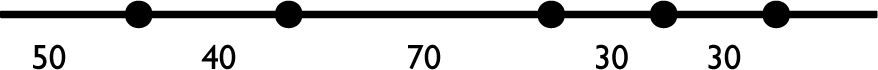
\includegraphics[width=0.65\textwidth]{images/00713.png}
  \caption{路点之间的相对距离示意}
  \label{fig:relative_dist_sample}
\end{figure}

图中的每个数字表示两个相邻圆点之间的距离。而我们期望程序计算出的结果如下图所示，其中每个圆点都标注了它到最左端起点的绝对距离：

\begin{figure}[htbp]
  \centering
  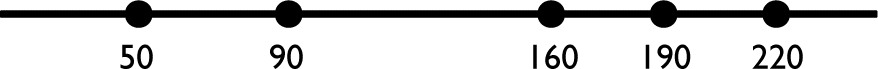
\includegraphics[width=0.65\textwidth]{images/00714.png}
  \caption{各路点相对于起点的绝对距离示意}
  \label{fig:absolute_dist_sample}
\end{figure}

按照常规的结构化设计配方，设计一个完成此计算的程序只是一次标准的基础练习。图 \ref{fig:177} 给出了完整的程序实现。当输入的列表不为 \code{\textquotesingle()} 时，自然递归调用会计算出 \code{(rest l)} 中其余圆点相对于列表首个测点的绝对距离。然而，由于列表中第一个测点本身并不是绝对原点（它与真正原点的距离为 \code{(first l)}），我们必须将 \code{(first l)} 累加到自然递归计算出的列表中的每一项上。这第二步——将一个固定数值加到数字列表的每个元素上——需要一个辅助函数 \code{add-to-each}。

\begin{figure}[htbp]
  \centering
\begin{lstlisting}[language=BSL, basicstyle=\scriptsize\ttfamily]
; [List-of Number] -> [List-of Number]
; converts a list of relative to absolute distances
; the first number represents the distance to the origin

(check-expect (relative->absolute '(50 40 70 30 30))
              '(50 90 160 190 220))

(define (relative->absolute l)
  (cond
    [(empty? l) '()]
    [else (local ((define rest-of-l
                    (relative->absolute (rest l)))
                  (define adjusted
                    (add-to-each (first l) rest-of-l)))
            (cons (first l) adjusted))]))

; Number [List-of Number] -> [List-of Number]
; adds n to each number on l

(check-expect (cons 50 (add-to-each 50 '(40 110 140 170)))
              '(50 90 160 190 220))

(define (add-to-each n l)
  (cond
    [(empty? l) '()]
    [else (cons (+ (first l) n) (add-to-each n (rest l)))]))
\end{lstlisting}
  \caption{将相对距离转换为绝对距离（结构型递归版本）}
  \label{fig:177}
\end{figure}

虽然设计这个程序直截了当，但在越来越长的列表上运行它却暴露出一个严重问题。考虑对以下表达式的求值：

\begin{lstlisting}[language=BSL]
(relative->absolute (build-list size add1))
\end{lstlisting}

随着 \code{size} 的增加，程序运行所需的时间呈现出急剧加速的态势：

\begin{table}[htbp]
  \centering
  \caption{函数 \code{relative->absolute} 在不同规模列表上的运行耗时（毫秒）}
  \label{fig:rel_abs_perf_table}
  \small
  \setlength{\tabcolsep}{3.5pt}
  \begin{tabular}{lrrrrrrr}
    \hline
    \code{size} & 1000 & 2000 & 3000 & 4000 & 5000 & 6000 & 7000 \\
    \hline
    \code{time} & 25 & 109 & 234 & 429 & 689 & 978 & 1365 \\
    \hline
  \end{tabular}
\end{table}

当列表规模从 1000 翻倍至 2000 时，运行耗时并没有相应翻倍，而是膨胀到了原来的近 4 倍；从 2000 增长到 4000 同样保持了约 4 倍的增速。借用插曲 5 中的渐近复杂度术语，我们称该函数的运行时间性能为 $\mathcal{O}(n^2)$，其中 $n$ 代表输入列表的长度。

\begin{notebox}[关于测量耗时的说明]
不同计算机与不同测试年份的实际运行耗时会有所差异。上表中的测试数据于 2017 年在一台运行 OS X 10.11 的 MacMini 上实测获得；而该书第一版早先于 1998 年所作的测量耗时要高出大约 100 倍。
\end{notebox}

\begin{exercise}{重构辅助函数 add-to-each}{489}
使用抽象函数 \code{map} 与 \code{lambda} 表达式重新表述辅助函数 \code{add-to-each}。
\end{exercise}

\begin{exercise}{推导 relative->absolute 的抽象运行时间公式}{490}
推导出一个数学公式，用以描述函数 \code{relative->absolute} 的抽象运行时间。

\textbf{提示}：手工逐步推导求值表达式：
\begin{lstlisting}[language=BSL]
(relative->absolute (build-list size add1))
\end{lstlisting}
从将 \code{size} 分别替换为 1、2 和 3 开始。每次求值过程中，分别需要调用多少次 \code{relative->absolute} 与 \code{add-to-each} 的递归？
\end{exercise}

考虑到问题本身的简单性，该程序所执行的庞大计算量令人十分吃惊。如果由人工在草稿纸上进行同样的转换，我们通常会一边沿着直线前行，一边维护当前走过的累计总距离，并将新遇到的相对距离顺次叠加进去即可。为什么计算机程序不能像人一样这样工作呢？

让我们尝试设计一个更贴近人工心算方法的函数版本。我们依然从标准的列表处理模板出发：

\begin{lstlisting}[language=BSL]
(define (relative->absolute/a l)
  (cond
    [(empty? l) ...]
    [else
     (... (first l) ...
      ... (relative->absolute/a (rest l)) ...)]))
\end{lstlisting}

现在让我们模拟一次单步手工推导演算：

\begin{lstlisting}[language=BSL]
  (relative->absolute/a (list 3 2 7))
== (cons ... 3 ... (relative->absolute/a (list 2 7)))
== (cons ... 3 ...
     (cons ... 2 ...
       (relative->absolute/a (list 7))))
== (cons ... 3 ...
     (cons ... 2 ...
       (cons ... 7 ...
         (relative->absolute/a '()))))
\end{lstlisting}

结果列表的第一个元素显然应该是 3，构造它毫无困难。但是，第二个元素应该是 \code{(+ 3 2)} 即 5，而第 2 个 \code{relative->absolute/a} 递归实例却根本无法“获知”原始列表的第一个元素是 3。这里的“知识”在递归深入的过程中被丢失了！

根本原因在于：\term{递归函数在本质上是独立于其上下文的}（context-independent）。在 \code{(cons N L)} 中对 \code{L} 的处理方式，与在 \code{(cons K L)} 中对 \code{L} 的处理方式完全一致；即便单独把 \code{L} 传入函数，处理过程也毫无二致。

为了弥补这一“上下文信息的丢失”，我们为函数增设一个额外的参数：\code{accu-dist}。该参数代表\term{累积距离}（accumulated distance），即我们在遍历相对距离列表转换为绝对距离列表时所持续记录的累计账目。其初始值必然为 0。随着函数在列表中逐项前进，它必须将每个路点的相对距离叠加到这个累加账目上。

修改后的函数定义如下：

\begin{lstlisting}[language=BSL]
(define (relative->absolute/a l accu-dist)
  (cond
    [(empty? l) '()]
    [else
     (local ((define tally (+ (first l) accu-dist)))
       (cons tally
             (relative->absolute/a (rest l) tally)))]))
\end{lstlisting}

递归调用接收列表的余下部分 \code{(rest l)} 以及当前路点相对于原点的新绝对距离 \code{tally}。尽管每次递归调用中两个参数都会发生变化，但第二个参数的更新严格依赖于第一个参数。该函数依然是一个纯粹的结构化列表处理程序。

现在让我们再次对其进行手工求值演算：

\begin{lstlisting}[language=BSL]
   (relative->absolute/a (list 3 2 7) 0)
== (cons 3 (relative->absolute/a (list 2 7) 3))
== (cons 3 (cons 5 (relative->absolute/a (list 7) 5)))
== (cons 3 (cons 5 (cons 12 ???)))
== (cons 3 (cons 5 (cons 12 '())))
\end{lstlisting}

\begin{notebox}[请停下来思考！]
请自行补全第 4 行中的问号处内容：此时调用的参数是什么？
\end{notebox}

上述手工求值清晰地揭示了引入累加器后转换过程得到了多大幅度的简化。列表中的每个项仅被访问和处理一次。当 \code{relative->absolute/a} 到达参数列表的末尾时，整个结果已经完全构建完毕，不再需要任何后续的二次遍历加工。一般而言，对于包含 $n$ 个元素的列表，该函数仅需执行约 $n$ 步自然递归。

然而这也带来了一个接口上的问题：与原函数 \code{relative->absolute} 相比，新函数需要两个参数，而非一个。更严重的是，调用者可能会不小心错误调用 \code{relative->absolute/a}，给它传入一个非 0 的累加初始值。我们可以借助局部定义 \code{local} 来封装 \code{relative->absolute/a}，同时解决这两个问题。图 \ref{fig:178} 展示了最终的优雅设计。现在，就输入-输出行为而言，\code{relative->absolute.v2} 与原先的 \code{relative->absolute} 完全等价。

\begin{figure}[htbp]
  \centering
\begin{lstlisting}[language=BSL, basicstyle=\scriptsize\ttfamily]
; [List-of Number] -> [List-of Number]
; converts a list of relative to absolute distances
; the first number represents the distance to the origin

(check-expect (relative->absolute.v2 '(50 40 70 30 30))
              '(50 90 160 190 220))

(define (relative->absolute.v2 l0)
  (local (
    ; [List-of Number] Number -> [List-of Number]
    (define (relative->absolute/a l accu-dist)
      (cond
        [(empty? l) '()]
        [else
          (local ((define accu (+ (first l) accu-dist)))
            (cons accu
                  (relative->absolute/a (rest l) accu)))])))
    (relative->absolute/a l0 0)))
\end{lstlisting}
  \caption{使用累加器转换相对距离}
  \label{fig:178}
\end{figure}

现在让我们来看看新版本的实际运行性能。为此，我们对下列表达式进行求值测试：

\begin{lstlisting}[language=BSL]
(relative->absolute.v2 (build-list size add1))
\end{lstlisting}

并将不同规模下的测试结果列于下表：

\begin{table}[htbp]
  \centering
  \caption{累加器版本 \code{relative->absolute.v2} 的耗时对比（毫秒）}
  \label{fig:rel_abs_v2_perf_table}
  \small
  \setlength{\tabcolsep}{5pt}
  \begin{tabular}{lrrrrrrr}
    \hline
    \code{size} & 1000 & 2000 & 3000 & 4000 & 5000 & 6000 & 7000 \\
    \hline
    \code{time} & 0 & 0 & 0 & 0 & 0 & 1 & 1 \\
    \hline
  \end{tabular}
\end{table}

令人惊叹的是，即便是处理包含 7000 个数字的长列表，\code{relative->absolute.v2} 的耗时也始终在 1 毫秒上下！对比前后两个版本的性能表现，你可能会误以为累加器是治愈所有程序性能迟缓的灵丹妙药。遗憾的是现实并非总是如此，但\textbf{只要一个结构型递归函数必须对其自然递归返回的结果进行递归式的二次加工}，你就应当毫不犹豫地考虑使用累加器。在此特定案例中，程序的时间复杂度从 $\mathcal{O}(n^2)$ 骤降至 $\mathcal{O}(n)$，并且常数项系数也得到了大幅削减。

\begin{exercise}{通过列表抽象重构相对距离转换}{491}
本书第一版的一位读者通过巧妙的设计构思，给出了针对该问题如下简洁的解法：

\begin{lstlisting}[language=BSL]
(define (relative->absolute l)
  (reverse
    (foldr (lambda (f l) (cons (+ f (first l)) l))
           (list (first l))
           (reverse (rest l)))))
\end{lstlisting}

该方案仅使用了 ISL+ 中大家熟知的内置函数：\code{reverse} 与 \code{foldr}（使用 \code{lambda} 仅是为了书写便利）。读者可能还记得，在本书第三部分中，\code{foldr} 本身正是依据前两部分的设计配方完全可设计出来的。

你朋友的这种简短解法是否意味着本节引入的复杂累加器设计纯属多余？有关解答请参阅第 \ref{sec:ch32_1} 节，但在翻阅之前，请先深入反思这个问题。\textbf{提示}：尝试自行设计 \code{reverse} 函数并分析其性能开销。
\end{exercise}

\section{生成型递归中的问题}
\label{sec:ch31_2}

接下来让我们重温在图（Graph）中沿路径“漫游”的问题：

\begin{notebox}[问题陈述：简单图中的路径连通性判定]
设计一个算法，检查一个简单图中的两个节点之间是否存在连通路径。在所谓的简单图中，每个节点有且仅有一条指向另一个节点（或指向自身）的有向连接。
\end{notebox}

第 29 章讨论了算法必须找出具体路径的复杂场景。本节的问题要更简单，因为我们的核心目标在于探讨该算法的累加器版本设计。

考查图 \ref{fig:179} 所示的样例图。图中共有从 A 到 F 的 6 个节点和 6 条有向连接。从 A 到 E 的路径必定经过 B 和 C。然而，从 A 出发到 F 则不存在任何连通路径；除 F 本身之外，也没有任何其他节点能到达 F。

\begin{figure}[htbp]
  \centering
  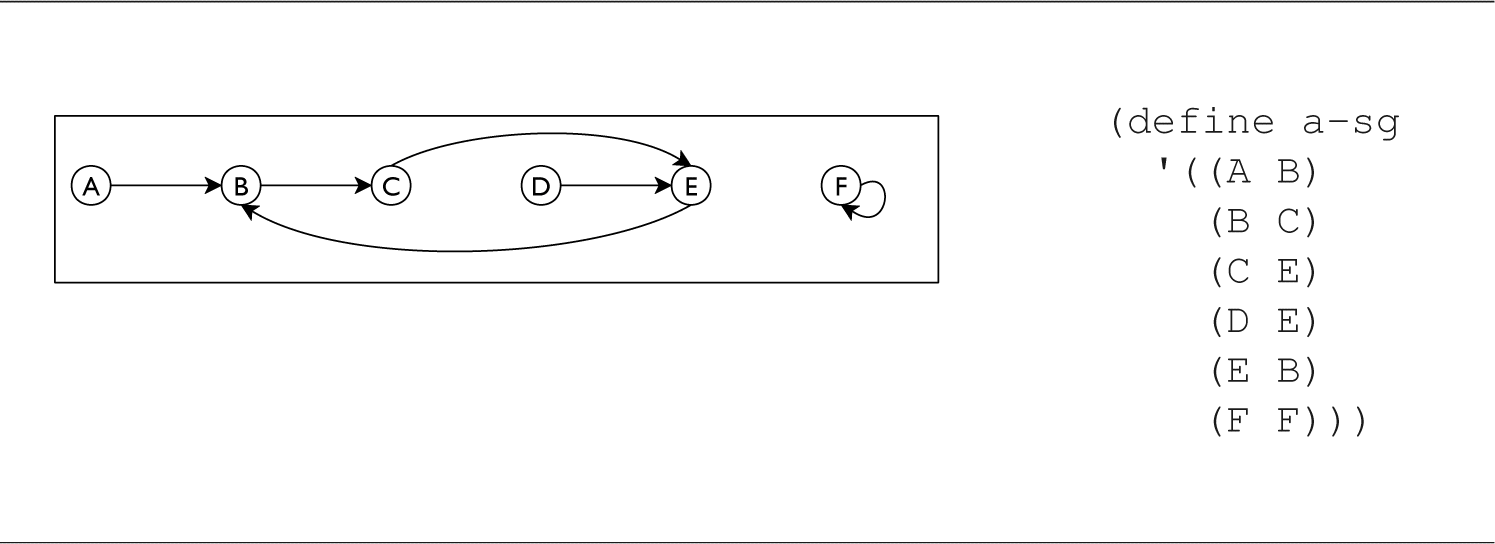
\includegraphics[width=0.85\textwidth]{images/00723.png}
  \caption{一个简单图及其在 BSL 中的嵌套列表表示}
  \label{fig:179}
\end{figure}

图 \ref{fig:179} 的右半部分展示了如何使用嵌套列表在程序中表示此图。每个节点表示为一个包含两个符号的列表：第一个符号是该节点的标签，第二个符号则是从该节点出发单步可达的目标节点。相关的数据定义如下：

\begin{lstlisting}[language=BSL]
; A SimpleGraph is a [List-of Connection]
; A Connection is a list of two items:
;   (list Node Node)
; A Node is a Symbol.
\end{lstlisting}

这些数据定义是我们非形式化描述的自然转译。我们已经知道该问题需要运用生成型递归，其函数签名、目的说明与测试用例很容易编写：

\begin{lstlisting}[language=BSL]
; Node Node SimpleGraph -> Boolean
; 判断在简单图 sg 中是否存在从 origin 到 destination 的路径
(check-expect (path-exists? 'A 'E a-sg) #true)
(check-expect (path-exists? 'A 'F a-sg) #false)
(define (path-exists? origin destination sg)
  #false)
\end{lstlisting}

接下来我们需要回答生成型递归设计配方的四个核心问题：
\begin{enumerate}
  \item \textbf{问题在何种情况下是平凡可解的？} 当起点 \code{origin} 与终点 \code{destination} 完全相同时，问题平凡。
  \item \textbf{平凡解是什么？} 解为 \code{\#true}。
  \item \textbf{在非平凡情况下如何生成新问题？} 若起点与终点不同，我们唯一能做的就是迈向起点的直接邻居节点，并从该邻居节点出发继续搜寻目标终点。
  \item \textbf{如何组合子问题的解？} 如果新问题找到了解，无需做额外组合变换：只要起点的邻居能够到达终点，起点本身就能到达终点；否则说明不存在连通路径。
\end{enumerate}

将上述答案转译为 ISL+ 代码，便得到了图 \ref{fig:180} 所示的完整程序。其中包括用于在简单图中查找某节点邻居的辅助函数 \code{neighbor}（这只是一个结构型递归的基础练习），以及覆盖两种可能输出结果的测试用例。

\begin{figure}[htbp]
  \centering
\begin{lstlisting}[language=BSL, basicstyle=\scriptsize\ttfamily]
; Node Node SimpleGraph -> Boolean
; is there a path from origin to destination in sg

(check-expect (path-exists? 'A 'E a-sg) #true)
(check-expect (path-exists? 'A 'F a-sg) #false)

(define (path-exists? origin destination sg)
  (cond
    [(symbol=? origin destination) #t]
    [else (path-exists? (neighbor origin sg)
                        destination
                        sg)]))

; Node SimpleGraph -> Node
; determine the node that is connected to a-node in sg
(check-expect (neighbor 'A a-sg) 'B)
(check-error (neighbor 'G a-sg) "neighbor: not a node")
(define (neighbor a-node sg)
  (cond
    [(empty? sg) (error "neighbor: not a node")]
    [else (if (symbol=? (first (first sg)) a-node)
              (second (first sg))
              (neighbor a-node (rest sg)))]))
\end{lstlisting}
  \caption{在简单图中寻找路径（初始生成型递归版本）}
  \label{fig:180}
\end{figure}

\begin{notebox}[警告：请勿贸然运行该程序！]
请不要直接运行该程序。如果你运行了，请时刻准备好用鼠标点击 DrRacket 的“Stop”按钮以中止程序死循环。事实上，哪怕只是粗略审视一下该函数，就能发现隐藏的严重缺陷：尽管规范要求当两点间无路径时产生 \code{\#false}，但程序代码中压根就没有任何返回 \code{\#false} 的分支！反过来我们必须追问：当两个节点之间确实不存在连通路径时，这个函数究竟在做什么？
\end{notebox}

请再次观察图 \ref{fig:179}。在图中，从 C 到 D 显然不存在路径。从 C 出发连线直接越过 D 通向了 E。让我们对 \code{(path-exists? \textquotesingle C \textquotesingle D a-sg)} 做一次手工推导演算：

\begin{lstlisting}[language=BSL]
   (path-exists? 'C 'D '((A B) ... (F F)))
== (path-exists? 'E 'D '((A B) ... (F F)))
== (path-exists? 'B 'D '((A B) ... (F F)))
== (path-exists? 'C 'D '((A B) ... (F F)))
\end{lstlisting}

推导确凿地证实：随着函数的不断递归，它以\textbf{完全相同的参数组合}一次又一次地反复调用自身！换言之，求值陷入了永无止境的死循环中。

这里暴露的问题再次归结为“上下文信息的丢失”，与前文的 \code{relative->absolute} 如出一辙。\code{path-exists?} 的设计同样假设递归调用与其历史上下文是彼此独立的。在此上下文中，这意味着该函数根本“不知道”在当前递归调用链条的前序步骤中，是否已经以完全相同的参数调用过自身。

解决这一设计困境的思路与上一节完全一致：我们为函数添加一个累加器参数，将其命名为 \code{seen}。它记录了从原始调用出发、当前递归链路上已经遭遇过的所有起点节点的列表。其初始值必然为 \code{\textquotesingle()}。当函数对某个特定的 \code{origin} 进行检查并转向其邻居节点时，\code{origin} 会被 \code{cons} 到 \code{seen} 的最前端。

以下是初步修改后的 \code{path-exists?/a}：

\begin{lstlisting}[language=BSL]
; Node Node SimpleGraph [List-of Node] -> Boolean
; 判断从 origin 到 destination 是否存在路径
; 假设：seen 中记录的所有节点均无法到达 destination
(define (path-exists?/a origin destination sg seen)
  (cond
    [(symbol=? origin destination) #true]
    [else (path-exists?/a (neighbor origin sg)
                          destination
                          sg
                          (cons origin seen))]))
\end{lstlisting}

仅添加这一参数本身尚不足以解决死循环问题，但正如对以下表达式的手工推导所示：

\begin{lstlisting}[language=BSL]
   (path-exists?/a 'C 'D '((A B) ... (F F)) '())
== (path-exists?/a 'E 'D '((A B) ... (F F)) '(C))
== (path-exists?/a 'B 'D '((A B) ... (F F)) '(E C))
== (path-exists?/a 'C 'D '((A B) ... (F F)) '(B E C))
\end{lstlisting}

它为终极解法奠定了坚实的基础！与原函数不同，修改后的函数在深入递归时不再以完全相同的参数调用自身。虽然在第 4 步调用中前三个常规参数再次与第 1 步相同，但累加器参数已迥然不同：它不再是 \code{\textquotesingle()}，而是 \code{\textquotesingle(B E C)}。这个新值明确告诉我们：在从 \code{\textquotesingle C} 到 \code{\textquotesingle D} 的搜索过程中，算法已经依次考察过 \code{\textquotesingle B}、\code{\textquotesingle E} 和 \code{\textquotesingle C} 作为起点了。

现在我们要做的，就是让算法充分利用这一累加的知识。具体而言，算法只需判断当前的 \code{origin} 是否已经包含在 \code{seen} 列表中。若是，说明路径出现环路陷入死循环，问题同样转化为平凡可解情形——其解直接判定为 \code{\#false}！图 \ref{fig:181} 给出了修正后的完整定义 \code{path-exists.v2?}，其中使用了 ISL+ 内置的谓词函数 \code{member?}。

\begin{figure}[htbp]
  \centering
\begin{lstlisting}[language=BSL, basicstyle=\scriptsize\ttfamily]
; Node Node SimpleGraph -> Boolean
; is there a path from origin to destination in sg

(check-expect (path-exists.v2? 'A 'E a-sg) #true)
(check-expect (path-exists.v2? 'A 'F a-sg) #false)

(define (path-exists.v2? origin destination sg)
  (local (; Node Node SimpleGraph [List-of Node] -> Boolean
          (define (path-exists?/a origin seen)
            (cond
              [(symbol=? origin destination) #t]
              [(member? origin seen) #f]
              [else (path-exists?/a (neighbor origin sg)
                                    (cons origin seen))])))
    (path-exists?/a origin '())))
\end{lstlisting}
  \caption{使用累加器在简单图中寻找路径}
  \label{fig:181}
\end{figure}

函数 \code{path-exists.v2?} 的封装同时消除了接口层面的一系列隐患：通过借助 \code{local} 局部化定义辅助函数，我们确保了首次调用时 \code{seen} 始终由 \code{\textquotesingle()} 干净启动；同时，主函数对外部调用者保持了原有的优雅签名与目的说明不变。

然而必须指出：\code{path-exists.v2?} 与前文的 \code{relative->absolute.v2} 之间存在着一个至关重要的质的飞跃。在相对距离的例子中，累加器版本与原版本在数学输入-输出映射上是严格等价的（只是运行速度千差万别）；但在有向图搜索中，原版函数在某些输入下会直接死循环崩溃，而\textbf{累加器版本则对任意给定的简单图都能正确终止并得出结论}！在这里，累加器不仅关乎效率，更是算法终止性与正确性的生命线。

\begin{exercise}{消除一般有向图中的死循环路径}{492}
修改图~\ref{fig:find-path-code}（原书图 169）中的路径判定定义，使得当算法在搜索过程中重复遭遇同一个起始节点时，程序能够正确终止并产生 \code{\#false}。
\end{exercise}
